We now introduce our system, called Text2KB, that expands upon the basic KBQA model by incorporating external textual sources throughout the QA process. The general architecture and an example use case of Text2KB is presented on Figure \ref{fig:model}. 
The left part of the figure roughly corresponds to the architecture of the existing information extraction approaches to KBQA, described above.
The right part introduces additional external text data sources, specifically
we investigate the use of web search results, community question answering (CQA) data, and a large collection of documents with detected KB entity mentions.
Recall that the main challenges in KBQA are linking topical entities in the question to the KB; identifying candidate answers in the neighborhood around the question entities; and ranking the candidates. In the rest of this section we present our approach to solving each of these challenges, by: using web search results, CQA data, and external corpus statistics. 


\subsection{Web search results for KBQA}
\label{section:method:web}

To obtain related web search results, Text2KB issues the question as a query to a commercial web search engine\footnote{https://datamarket.azure.com/dataset/bing/search}, extracts top 10 search result snippets and the corresponding documents.
Next, it detects KB entity mentions in both snippets and documents.
% Document snippets are usually built to present the information most relevant to the query, and often contain answers to a question.
% Unfortunately, for longer queries the snippets often represent and combination of small phrases, that contain mostly question terms and very few additional information.
% Nevertheless, we keep both snippets and documents text, and using thesystem's linker detect KB entity mentions.
This data turns out to be useful for multiple purposes, \ie question entity identification and answer candidate ranking.

\textbf{Question entity identification}.
Question text provides only a limited context for entity disambiguation and linking; additionally, the entity name can be misspelled or an uncommon variation used.
This complicates the task of entity identification, which is the foundation of whole question answering process.
Fortunately, web search results help with these problems, as they usually contain multiple mentions of the same entities and provide more context for disambiguation.
Text2KB uses the search result snippets to {\em expand} the set of detected question entities.
To keep only the entities that are also mentioned in the question and avoid irrelevant entities, we use string distance.
More specifically, we take names of all entities detected in the question and compute their term by term similarity with non-stopwords from the question.
In this work we used Jaro-Winkler string distance and entity was added to the list of question entities if at least one of its tokens $e_t$ has high similarity with one of the question tokens $q_t$ excluding stopwords ($Stop$):
$$\max_{e_t \in M\backslash Stop, q_t \in Q\backslash Stop} distance_{Jaro-Winkler}(e_t, q_t) \geq 0.8$$

\textbf{Answer candidate features}.
Most of the information stored in knowledge bases is also present in other formats, including natural language statements, tables, \etc
For example, on Figure \ref{fig:web_search_entitylink} multiple snippets mention the date when Tutankhamun became the king.
Text-QA systems usually generate answer candidates from passages extracted from retrieved documents.
In our case candidates are already generated from a KB and we just need to rank them to select the best one.
Text2KB uses snippets and documents to compute a set of features, which are used for answer candidate ranking.
More specifically we do this following:

\vspace{-0.2cm}
\begin{enumerate}
\setlength\itemsep{-0.5em}
\item Precompute term and entity IDFs\footnote{https://en.wikipedia.org/wiki/Tf-idf}. We used Google n-grams corpus to approximate terms IDF by collection frequencies and available ClueWeb Freebase entity annotations\footnote{http://lemurproject.org/clueweb09/FACC1/} to compute entity IDFs
\item Each snippet and document is represented by two TF-IDF vectors of lowercased tokens and mentioned entities
\item In addition, vectors of all snippets and all documents are merged together to form combined token and entity vectors
\item Each answer candidate is also represented as TF-IDF vectors of terms (from entity names) and entities
\item We compute cosine similarities between answer and each snippet and document token and entity vectors. This gives us 10 similarity scores for every document for token vectors and 10 similarities for entity vectors, we take average and maximum scores as features.
\item We do the same for the combined document and use cosine similarities as features.
\end{enumerate}

\subsection{CQA data for Matching Questions to Predicates}
\label{section:method:cqa}

Recall that a major challenge in KBQA is that natural language questions do not easily or uniquely map to entities and predicates in a KB. An established approach for this task is supervised machine learning, which requires labeled examples of questions and the corresponding answer to learn this mapping. Unfortunately, manual labeling of questions with answers is expensive, and necessarily contains only a small fraction of the different ways the same KB predicate can be inquired about using natural language questions. Researchers have proposed to use weakly supervised methods to extend the lexicon with mappings learned from \textit{single sentence statements} mentioning entity pairs from a large corpus \cite{yao2014information}.
However, often there is a lexical gap between how information is asked about in a question and how it is expressed in a statement.
On the other hand there are huge archives of questions and answers posted by real users on various community question answering websites, \eg Figure \ref{fig:cqa_example}.

\begin{figure}
\centering
\fbox{
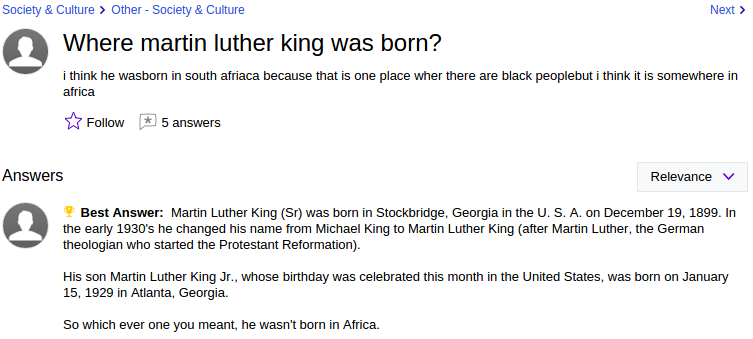
\includegraphics[width=0.45\textwidth]{img/cqa_example}
}
\vspace{-0.5cm}
\caption{Example of a question and answer pair from Yahoo! Answers CQA website}
\label{fig:cqa_example}
\vspace{-0.4cm}
\end{figure}

For our experiments we use 4,483,032 questions from Yahoo! Comprehensive Questions and Answers WebScope dataset\footnote{https://webscope.sandbox.yahoo.com/catalog.php?datatype=l}.
Texts of each question and answer pair were run through an entity linker, that detected mentions of Freebase entities.
Next, similar to an idea of relation extraction from CQA data \cite{savenkov-EtAl:2015:SRW}, we use distant supervision to label each question-answer pair with predicates between entities mentioned in the question and in the answer.
As a result, we have a set of questions, annotated with KB predicates, which are, often incorrectly, assumed to answer the question.
We learn the associations between question terms and predicates by computing pointwise mutual information scores\footnote{https://en.wikipedia.org/wiki/Pointwise\_mutual\_information} (PMI) for each term-predicate pair.
Examples of scores for some terms from WebQuestions dataset questions are given in Table \ref{table:cqa_npmi}.

\begin{table}
\caption{Examples of term-predicate pairs with high PMI scores, computed using distant supervision from a CQA collection}
\label{table:cqa_npmi}
\begin{tabular}{| p{1cm} | p{5.5cm} | p{0.75cm} |}
\hline
Term & Predicate & PMI score\\
\hline
born & people.person.date\_of\_birth & 3.67\\
 & people.person.date\_of\_death & 2.73\\
 & location.location.people\_born\_here & 1.60\\
\hline
kill & people.deceased\_person.cause\_of\_death & 1.70\\
& book.book.characters & 1.55\\
\hline
currency & location.country.currency\_formerly\_used & 5.55 \\
& location.country.currency\_used & 3.54 \\
\hline
school & education.school.school\_district & 4.14 \\
& people.education.institution & 1.70\\
& sports.school\_sports\_team.school & 1.69 \\
\hline
illness & medicine.symptom.symptom\_of & 2.11\\
& medicine.decease.causes & 1.68\\
& medicine.disease.treatments & 1.59\\
\hline
win & sports.sports\_team.championships & 4.11\\
& sports.sports\_league.championship & 3.79\\
\hline
\end{tabular}
\end{table}

Although noisy, the statistics look reasonable to be used for candidate ranking.
In Text2KB we take candidate answer predicates and look up the  PMI scores between these predicates and terms in the question.
Missing pairs are given a score of 0, and minimum, average and maximum of these scores are used as features.
Since this kind of data is usually sparse, we also use pretrained word2vec word embeddings\footnote{https://code.google.com/p/word2vec/} to generate predicate embeddings by taking weighted average of term vectors from predicate's PMI table.
Each term's embedding vector is weighted by its PMI value (terms with negative score are skipped).
Then, we compute cosine similarities between predicate vector and question term vectors and take their minimum, average, maximum as features.
Similarity between the predicate vector and average question term vector is also computed.


\subsection{Estimating Entity Associations}
\label{section:method:clueweb}

When ranking candidate answers, we are interested in estimating whether the entities in the question and the answer are related in a way asked in the question.
Existing systems usually look on how candidate predicates are expressed in questions and statements.
But predicate isn't the only way we can look at this. An alternative is to consider text passages, \eg sentences, that mention topical and answer entities together.
For example, in the bottom right corner of Figure \ref{fig:model} we can see some passages that mentioned a pair of people, and the context of these mentions often expresses the nature of the relationships between the entities.

We use the ClueWeb12 corpus with existing Freebase entity annotations\footnote{http://lemurproject.org/clueweb12/FACC1/} and compute counts of different terms that occur in the context to an entity pair mention.
By an entity pair mention we mean a pair of mentions of different entities within 200 characters of each other.
We take terms in between mentions and 100 character before and after mentions as the context.
A small sample of this data is presented in Table \ref{table:clueweb_entitypairs_langmodel}.

\begin{table}
\caption{Example of entity pairs along with the most popular terms mentioned around the entities}
\label{table:clueweb_entitypairs_langmodel}
\begin{tabular}{| p{1.25cm} | p{1.23cm} | p{4.5cm} |}
\hline
Entity 1 & Entity 2 & Term counts\\
\hline
John Edwards & Rielle Hunter & campaign, affair, mistress, child, former ...\\
\hline
John Edwards & Cate Edwards & daughter, former, senator, courthouse, left, greensboro, eldest ...\\
\hline
John Edwards & Elizabeth Edwards & wife, hunter, campaign, affair, cancer, rielle, husband ...\\
\hline
John Edwards & Frances Quinn Hunter & daughter, john, rielle, father, child, former, paternity...\\
\hline
\end{tabular}
\end{table}

First, given a set of question terms $Q$ and an answer candidate, that starts from a question entity $e_1$, we compute a language model score for every answer entity $e_2$:
$$p(Q|e_1, e_2) = \prod_{t\in Q} p(t | e_1, e_2)$$
and use minimum, average and maximum as features.
To address the sparsity problem, we again use embeddings, 
ie for each entity pair a weighted (by counts) average embedding vector of terms is computed and minimum, average and maximum cosine similarities between these vectors and question tokens vector are used as features.

\subsection{Internal text data to enrich entity representation}
In addition to external text data, many knowledge bases, including Freebase, contain text data as well.
In Freebase, most of the entities contain a description paragraph, which often comes from the entity Wikipedia profile.
These descriptions of entities in the KB were found useful for text-based question answering \cite{Sun:2015:ODQ:2736277.2741651}.
For completeness, we include them in our system. The aim is to improve the matching of the question text, to the unstructured description of the candidate entities. For this, each entity description is represented as a vector of tokens, and a vector of mentioned entities. We compute cosine similarities between the question tokens and each of the candidate entity vectors, and use these scores as features for candidate ranking.
In future work, we could explore incorporating any other entity profile text, such as full Wikipedia article.



